\section{Grundlagen des RadarImagers}

\begin{figure}[htbp]
    \centering
      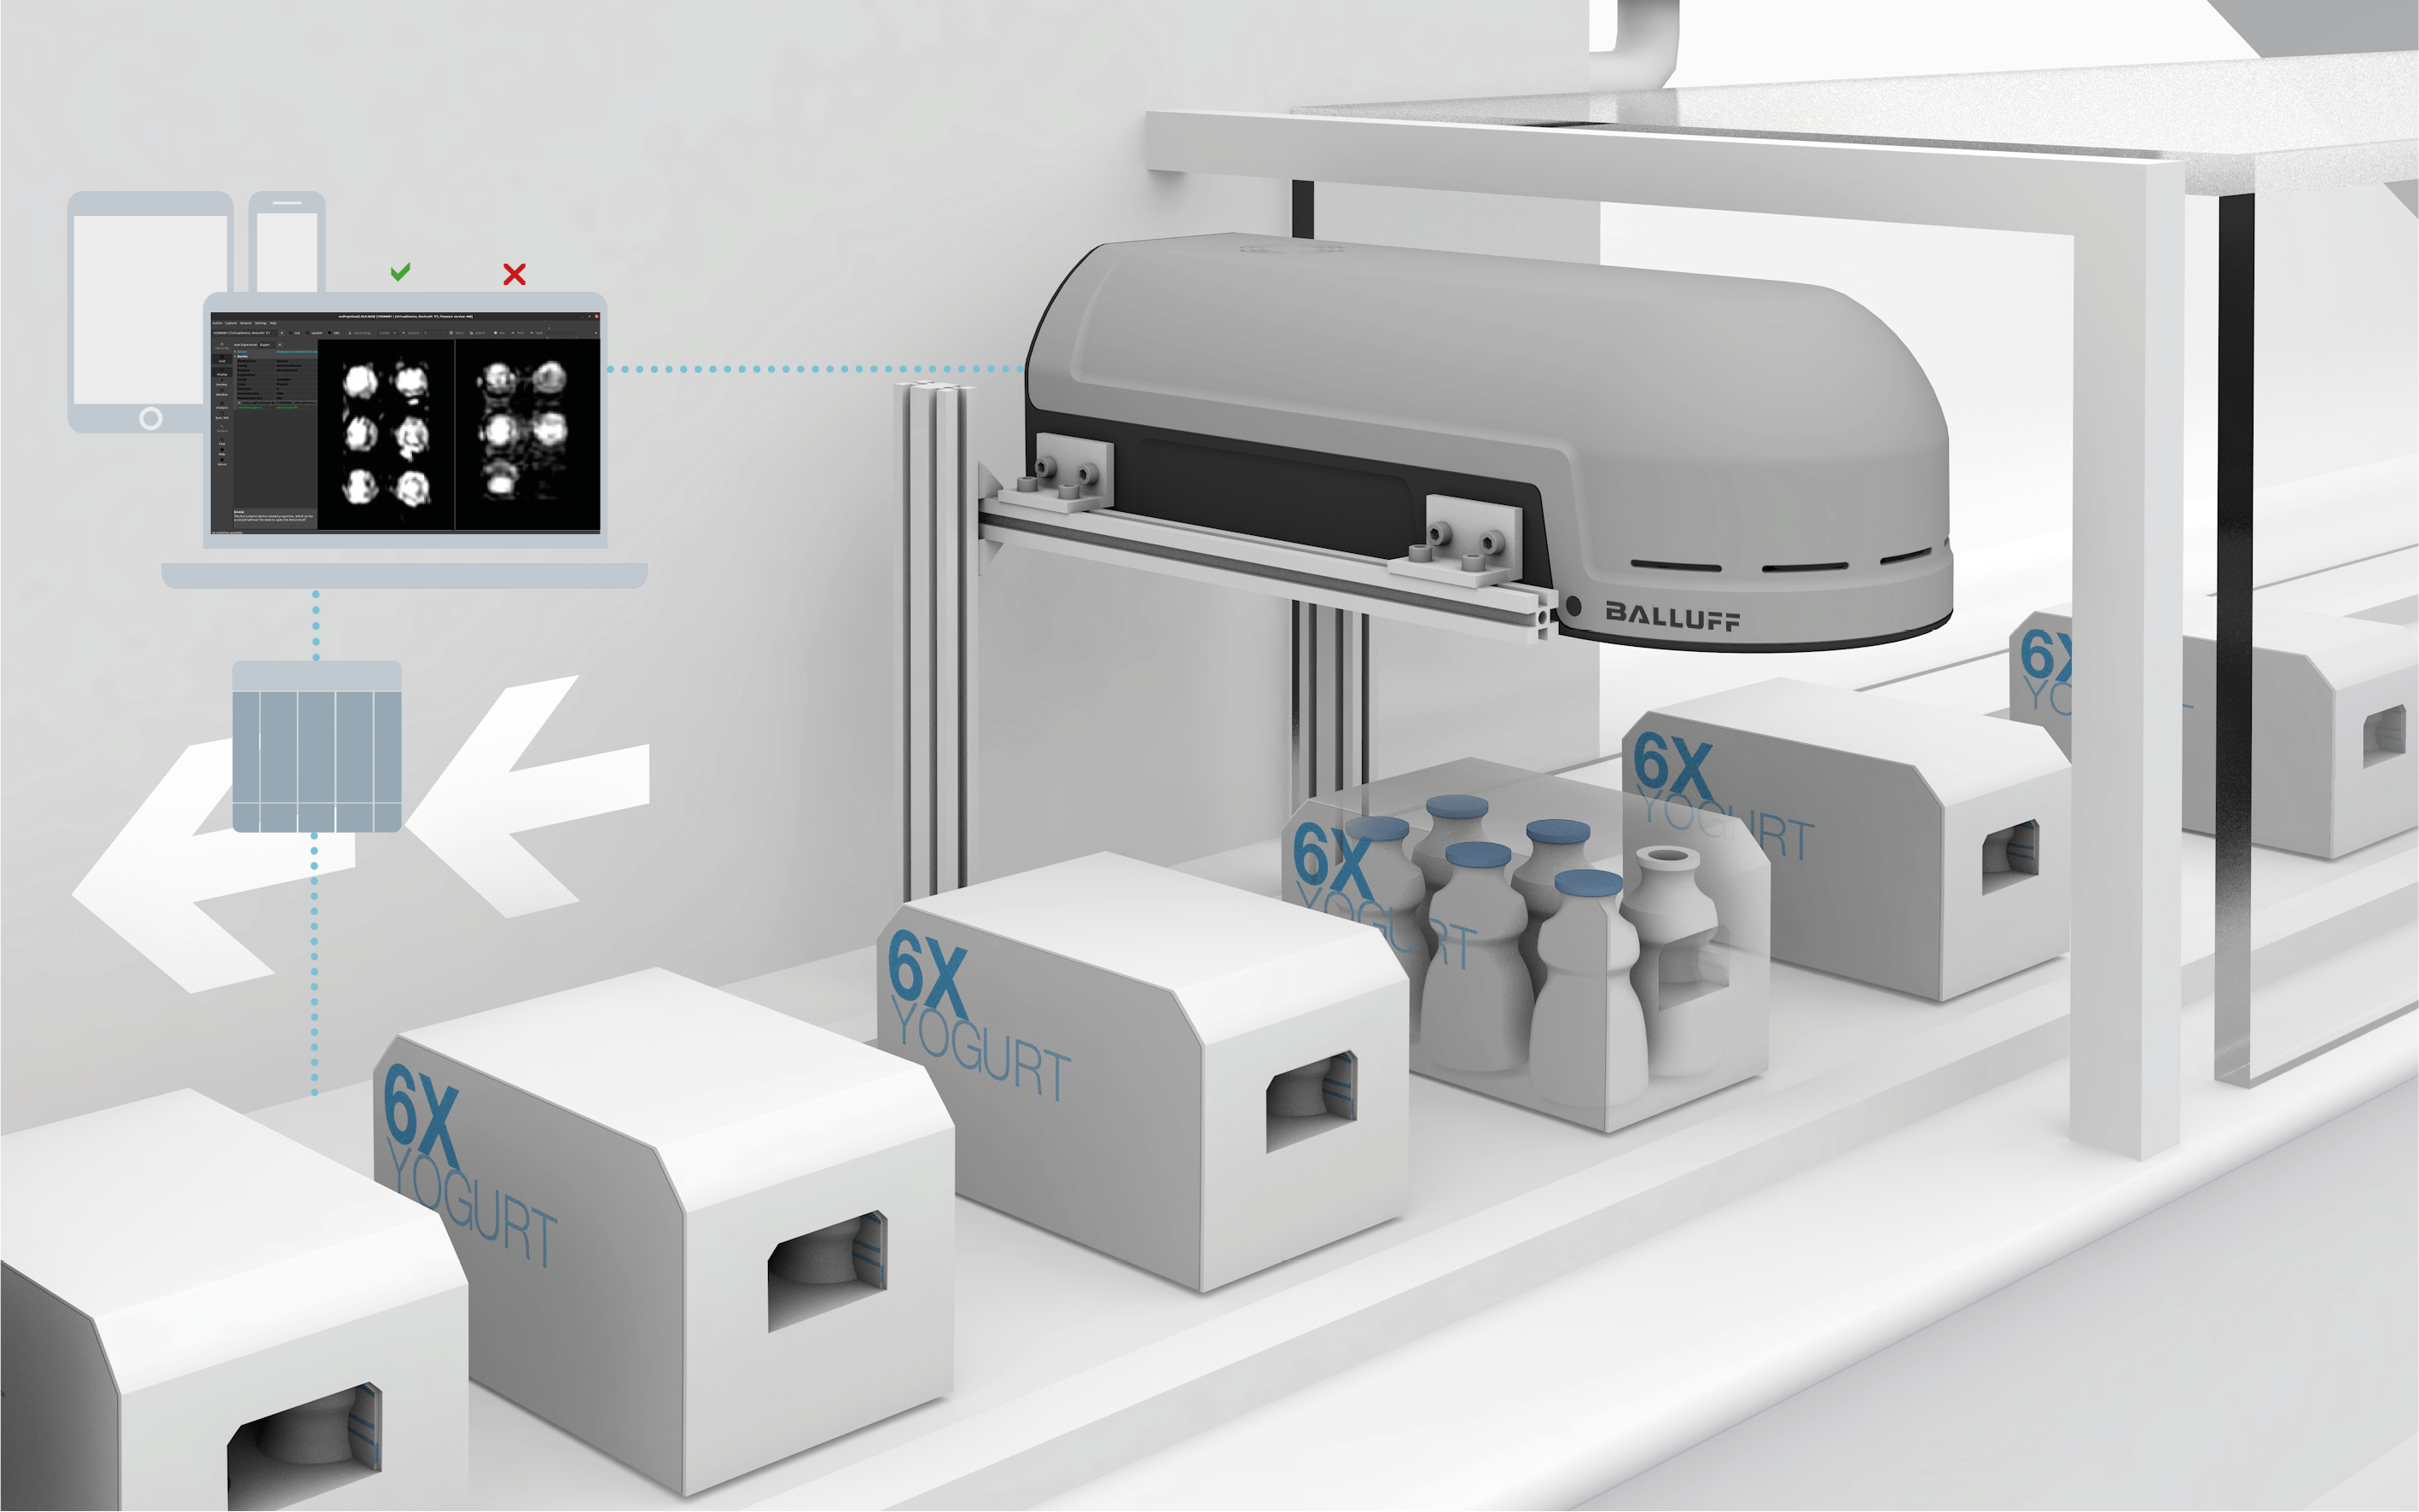
\includegraphics [width=0.8\textwidth]{RadarImager.jpg}
    \caption[RadarImager]{RadarImager \citep{BalluffRIPressekit}}
    \label{fig:RadarImager}
\end{figure}

Der RadarImager von Balluff ist ein industrielles 3D-Bildgebungssystem, welches Objekte hinter nicht-leitfähigen Materialien sichtbar macht. 
Dieses System findet Anwendung in der Qualitätssicherung, insbesondere in Branchen wie der Verpackungs- und Pharmaindustrie. Es ermöglicht 
eine zerstörungsfreie Kontrolle von Verpackungen auf Vollständigkeit, die Überprüfung der Unversehrtheit des Produkts sowie die Identifizierung von Fremdkörpern. 
Darüber hinaus können Verschlüsse geprüft und Füllstände erkannt werden (siehe Abbildung \ref{fig:RadarImager}). Die Auswertung der Bilder 
erlaubt die zuverlässige Identifikation von Fehlern.

Der RadarImager basiert auf der Radartechnologie, wobei Radar für \glqq Radio Detection And Ranging\grqq\ steht. Diese Technologie nutzt elektromagnetische Wellen, 
um Informationen über die Position, Bewegung und Eigenschaften von Objekten zu erhalten. Das System sendet elektromagnetische Wellen aus, die von den 
Objekten reflektiert oder absorbiert werden. Der Frequenzbereich 
der verwendeten Radarwellen liegt im elektromagnetischen Spektrum zwischen Mikrowelle und Infrarot, somit im unteren Gigahertz-Bereich. In diesem 
Frequenzbereich sind die Wellen nicht ionisierend, sodass keine gesundheitlichen Risiken bestehen. Die Wellenenergie wird je nach Material spezifisch 
absorbiert, was zu einer Reduzierung der Amplitude führt. Die Reflektion an den Grenzflächen der Objekte resultiert in Laufzeitdifferenzen zwischen der 
ursprünglichen und der reflektierten Welle. Die reflektierten Wellen werden vom RadarImager empfangen und anschließend als Signale aufbereitet, verarbeitet und analysiert.
Eine Software wandelt diese Signale im Anschluss in Bilder um, die für das menschliche Auge erkennbar und somit auswertbar sind. Der RadarImager kann sämtliche dielektrische Materialien wie Folien, Kartonagen und 
Kunststoffe durchleuchten. Leitfähige Gegenstände, Metall und Flüssigkeiten werden erkannt, aber nicht durchdrungen. Daher können auch metallische 
Objekte aufgefunden und Füllstände gemessen werden. 

\begin{figure}[htbp]
  \centering
    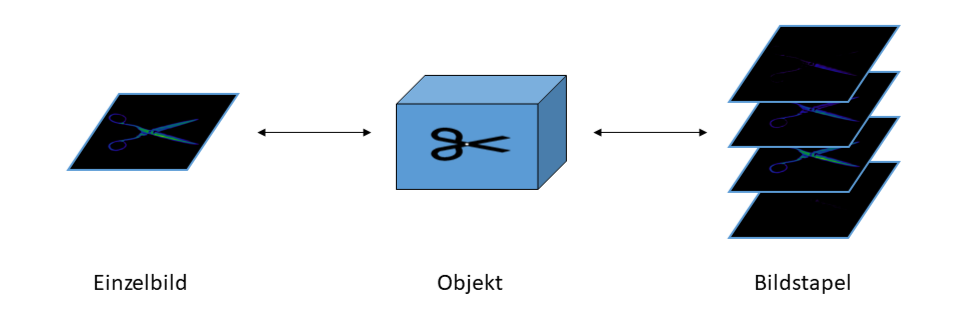
\includegraphics [width=1\textwidth]{Bildstapel.png}
  \caption[Einzelbild und Bildstapel]{Einzelbild und Bildstapel (eigene Darstellung)}
  \label{fig:Bildstapel}
\end{figure}

Der RadarImager ermöglicht es, zwischen Einzelbildern oder mehreren Bildern einer Messung (sogenannten Bildstapeln) zu wählen (siehe Abbildung \ref{fig:Bildstapel}). Ein Bildstapel ist eine 
Sammlung von Schichtaufnahmen, ähnlich den Ergebnissen einer MRT-Untersuchung in der Medizin. Dies ermöglicht es, später gezielt die Schichten mit dem höchsten Informationsgehalt 
auszuwählen oder mehrere Schichten gleichzeitig zu analysieren. Die Bilder werden mithilfe von GenICam
über Gigabit-Ethernet übertragen. Dabei wird das GigE Vision Protokoll für die Kommunikation und den Datentransfer verwendet.
Der RadarImager verfügt über eine 12V-Spannungsversorgung sowie zwei Eingänge für Trigger. Der erste Eingang ist für die Objekterkennung und die Erstellung 
des Bildes vorgesehen. Der zweite Eingang kann zur Messung der Bewegungsrichtung und Geschwindigkeit des Objekts verwendet werden. Des Weiteren ist ein 
Ethernet-Anschluss (RJ45) für die Übertragung der Bilder vorhanden und LEDs, die zur Anzeige des Zustands dienen. 

\citep{BalluffRIPressekit}